\documentclass{article}

% if you need to pass options to natbib, use, e.g.:
\PassOptionsToPackage{numbers, compress}{natbib}
% before loading neurips_2019

% ready for submission
\usepackage[final]{neurips_2019}

% to compile a preprint version, e.g., for submission to arXiv, add add the
% [preprint] option:
%     \usepackage[preprint]{neurips_2019}

% to compile a camera-ready version, add the [final] option, e.g.:
% \usepackage[final]{neurips_2019}

% to avoid loading the natbib package, add option nonatbib:
%     \usepackage[nonatbib]{neurips_2019}

\usepackage[utf8]{inputenc} % allow utf-8 input
\usepackage[T1]{fontenc}    % use 8-bit T1 fonts
\usepackage{hyperref}       % hyperlinks
\usepackage{url}            % simple URL typesetting
\usepackage{booktabs}       % professional-quality tables
\usepackage{amsfonts}       % blackboard math symbols
\usepackage{nicefrac}       % compact symbols for 1/2, etc.
\usepackage{microtype}      % microtypography
% Better maths.
\usepackage{amsmath,amsthm,amssymb,bm,mathtools}
% If possible, it is preferable to directly include PDF images.
\usepackage{graphicx}
\graphicspath{{fig/}}

%% Macros.

% "Transpose" symbol.
\newcommand{\tr}{^\intercal}
% Email.
\newcommand{\email}[1]{\href{mailto:#1}{\nolinkurl{#1}}}
% Arg{sort, min, max}.
\DeclareMathOperator*{\argsort}{arg\,sort}
\DeclareMathOperator*{\argmax}{arg\,max}
\DeclareMathOperator*{\argmin}{arg\,min}
% Shortcut CO\textsubscript{2}.
\newcommand\COtwo{CO\textsubscript{2}}
% "Given" symbol.
% \newcommand\given{\:\vert\:}
\newcommand\given{\;|\;}
% Vectors in bold
\renewcommand{\vec}[1]{\boldsymbol{#1}}
% Enumerate with bold numbers.
\newenvironment{enumerateb}
{\begin{enumerate}\renewcommand\labelenumi{\textbf\theenumi .}}
		{\end{enumerate}}
% An action item for the list.
\newcommand{\actiontitle}[1]{\textbf{#1}}
\newcommand{\actionvalue}[1]{\textbf{Carbon footprint:} #1 kg\COtwo-equivalent.}

% Paper title.
\title{A User Study of Perceived Carbon Footprint}

% The \author macro works with any number of authors. There are two commands
% used to separate the names and addresses of multiple authors: \And and \AND.
%
% Using \And between authors leaves it to LaTeX to determine where to break the
% lines. Using \AND forces a line break at that point. So, if LaTeX puts 3 of 4
% authors names on the first line, and the last on the second line, try using
% \AND instead of \And before the third author name.

\author{%
	Victor Kristof\\
	EPFL
	% \texttt{victor.kristof@epfl.ch} \\
	% examples of more authors
	\And
	Valentin Quelquejay-Leclère \\
	EPFL
	% \texttt{lucas.maystre@spotify.com} \\
	\And
	Robin Zbinden \\
	EPFL
	% \texttt{lucas.maystre@spotify.com} \\
	\AND
	Lucas Maystre \\
	Spotify
	% \texttt{lucas.maystre@spotify.com} \\
	\And
	Matthias Grossglauser \\
	EPFL
	% \texttt{matthias.grossglauser@epfl.ch} \\
	\And
	Patrick Thiran \\
	EPFL
	% \texttt{patrick.thiran@epfl.ch} \\
}

\begin{document}

\maketitle

% Max 250 wrods, c.f. https://wordcounter.net/.
As the number of contributors to online peer-production systems grows, it becomes increasingly important to predict whether the edits that users make will eventually be beneficial to the project.
Existing solutions either rely on a user reputation system or consist of a highly specialized predictor that is tailored to a specific peer-production system.
In this work, we explore a different point in the solution space that goes beyond user reputation but does not involve any content-based feature of the edits.
We view each edit as a game between the editor and the component of the project.
We posit that the probability that an edit is accepted is a function of the editor's skill, of the difficulty of editing the component and of a user-component interaction term.
Our model is broadly applicable, as it only requires observing data about \emph{who} makes an edit, \emph{what} the edit affects and whether the edit survives or not.
We apply our model on Wikipedia and the Linux kernel, two examples of large-scale peer-production systems, and we seek to understand whether it can effectively predict edit survival:
in both cases, we provide a positive answer.
Our approach significantly outperforms those based solely on user reputation and bridges the gap with specialized predictors that use content-based features.
It is simple to implement, computationally inexpensive, and in addition it enables us to discover interesting structure in the data.

%We apply it to Wikipedia and the Linux kernel, two examples of large-scale collaborative projects.
%In both cases, the model enables us (a) to discover interesting structure in the data and (b) to effectively predict whether edits will survive.

%! TEX root = ../thesis.tex
\section{Introduction}
\label{lmp:sec:intro}

The process of maintaining a body of law in a democratic society shares many features with peer-production systems.
The work of parliaments is governed by complex rules, processes, and conventions, in order to foster compromises among competing viewpoints and priorities.
How well this process works, to what extent it is subject to biases and to benign or undue influences is of obvious concern to citizens and to scientists alike.
An exciting recent development in this regard is the adoption of {\em open government initiatives}, such as in the United States~\citep{open2009barack}, Switzerland~\citep{switzerland2021open}, Brazil~\citep{brazil2021dado}, and the European Union~\citep{european2021data}.
Open-government data published on the Web are of great interest to citizens, companies, sub- and supra-government entities, and researchers.
These initiatives aim to improve the transparency of the law-making process and the accountability of its protagonists.

Not surprisingly, the dynamics of this process is complex, given the confluence of many stakeholders, topics, special interests, and lobbying groups.
Until open-government was introduced, the work of parliaments had not been systematically accessible to the general public, and internal documents -- when they existed -- were difficult to find.
The European Union (EU), however, has been a pioneer in opening the mechanics of its parliament.
It publishes detailed records of the process by which bills are written and amended, until they finally become law.
Once an initial draft of a new law has been published, parliamentarians (MEPs, for Members of the European Parliament) in one or several specialized committees examine the draft and propose amendments.
Several amendments can be in conflict if they attempt to modify the same part of the law draft.
To be instituted, an amendment needs to be approved by the committee in charge, and ultimately by the full plenary.
The European Parliament publishes every proposed amendment and its authorship, along with various other details.
This makes it possible to build detailed models of the interplay between MEPs, laws, amendments, and committees.

In this work, we (i) curate a large-scale dataset of amendments proposed by MEPs over two legislature periods (2009--2019) and (ii) develop a predictive model for the success and failure of proposed amendments.
Specifically, we collect explicit features for each MEP, including their party membership, country of origin, and gender.
We also collect explicit features of the amendments and dossiers (law drafts), including  their type and the committee in charge.
Finally, we extract the actual text of the amendments, which consists of \emph{edits} of the proposed law.
Our dataset contains \numprint{449493} edits proposed by \numprint{1214} parliamentarians on \numprint{1889} dossiers

Our model relies mostly on the structure of incompatible edits, which can be viewed as a {\em conflict graph} among all edits that target the same law.
We posit a measure of {\em strength} for each parliamentarian, and an edit inherits the strengths of its supporters.
There are two sources of competition in the process.
First, a proposed edit competes with the status quo, because the edit can be rejected in favor of not changing the existing state of a law.
Our model incorporates this by endowing each law with a measure of {\em inertia} that represents the level of controversy of a law.
Second, proposed edits of a law are frequently mutually exclusive, because they overlap and are incompatible.
These edits then compete against each other, as well as against the status quo.

We further include explicit features and text features into the model.
This combination gives rise to models with improved predictive performance and enables us to make predictions for unseen laws.
We also endow our model with a set of latent features for both laws and MEPs, which capture richer interactions between them.
Indeed, it would seem plausible that an MEP might be an expert in one subject matter, but less knowledgeable in another, which would bear upon their effectiveness in promoting a particular amendment.

% TODO: Adapt with new sections.
The remainder of this chapter is structured as follows.
In Section~\ref{lmp:sec:dataset}, we state the problem and provide a detailed description of our dataset.
We describe our statistical models in Section~\ref{lmp:sec:models}.
We give the results and interpretations of our experiments in Section~\ref{lmp:sec:results}.
We describe related work in Section~\ref{lmp:sec:relwork} and conclude in Section~\ref{lmp:sec:conclusion}.

%! TEX root = ../thesis.tex
\section{Model}
\label{kks:sec:model}

% Introduction to the section.
In this section, we formally introduce our probabilistic model.
For clarity, we take a clean-slate approach and develop the model from scratch.
We discuss in more detail how it relates to prior work in Section~\ref{kks:sec:relwork}.

% Features have latent score process that follows a GP
The basic building blocks of our model are \emph{features}\footnote{%
	In the simplest case, there is a one-to-one mapping between competitors (e.g., teams) and features, but decoupling them offers increased modeling power.}.
Let $M$ be the number of features; each feature $m \in [M]$ is characterized by a latent, continuous-time Gaussian process
\begin{align}
	\label{kks:eq:score}
	s_m(t) \sim \GP[0, k_m(t, t')].
\end{align}
We call $s_m(t)$ the \emph{score process} of $m$, or simply its \emph{score}.
The \emph{covariance function} of the process, $k_m(t, t') \doteq \Exp{s_m(t) s_m(t')}$, is used to encode time dynamics.
A brief introduction to Gaussian processes as well as a discussion of useful covariance functions is given in Section~\ref{kks:sec:covariances}.
The $M$ scores $s_1(t), \dots, s_M(t)$ are assumed to be (a priori) jointly independent, and we collect them into the \emph{score vector}
\begin{align*}
	\bm{s}(t) = \begin{bmatrix}s_1(t) & \cdots & s_M(t) \end{bmatrix}\Tr.
\end{align*}

% Competitors are sparse linear combination of M features
For a given match, each opponent $i$ is described by a sparse linear combination of the features, with coefficients $\bm{x}_i \in \mathbf{R}^M$.
That is, the score of an opponent $i$ at time $t^*$ is given by
\begin{align}
	\label{kks:eq:compscore}
	s_i = \bm{x}_i\Tr \bm{s}(t^*).
\end{align}
In the case of a one-to-one mapping between competitors and features, $\bm{x}_i$ is simply the one-hot encoding of opponent $i$.
More complex setups are possible: For example, in the case of team sports and if the player lineup is available for each match, it could also be used to encode the players taking part in the match \citep{maystre2016player}.
Note that $\bm{x}_i$ can also depend contextually on the match.
For instance, it can be used to encode the fact that a team plays at home \citep{agresti2012categorical}.

% Observations are parametrized by score difference.
Each observation consists of a tuple $(\bm{x}_i, \bm{x}_j, t^*, y)$, where $\bm{x}_i, \bm{x}_j$ are the opponents' feature vectors, $t^* \in \mathbf{R}$ is the time, and $y \in \mathcal{Y}$ is the match outcome.
We posit that this outcome is a random variable that depends on the opponents through their latent score difference:
\begin{align*}
	y \mid \bm{x}_i, \bm{x}_j, t^* \sim p( y \mid s_i - s_j ),
\end{align*}
where $p$ is a known probability density (or mass) function and $s_i, s_j$ are given by~\eqref{kks:eq:compscore}.
The idea of modeling outcome probabilities through score differences dates back to \citet{thurstone1927law} and \citet{zermelo1928berechnung}.
The likelihood $p$ is chosen such that positive values of $s_i - s_j$ lead to successful outcomes for opponent $i$ and vice-versa.

% Graphical representation.
A graphical representation of the model is provided in Figure~\ref{kks:fig:pgms}.
For perspective, we also include the representation of a static model, such as that of \citet{thurstone1927law}.
Our model can be interpreted as ``conditionally parametric'': conditioned on a particular time, it falls back to a (static) pairwise-comparison model parametrized by real-valued scores.

\begin{figure}[t]
	\subcaptionbox{
		Static model
	}[2cm]{
		\begin{tikzpicture}

% Nodes.
\node[latent] (s)  {$s_m$};
\node[obs, below=of s] (y) {$y_n$};
\node[const, left=0.3cm of y, yshift=0.4cm] (x) {$\bm{x}_n$};

% Edges.
\edge {s} {y};
\edge[-] {x} {y};

% Plates.
\plate {scores} {(s)} {$M$}
\plate {observations} {(y)(x)} {$N$}
\end{tikzpicture}

	}
	\hfill
	\subcaptionbox{
		Our dynamic model \label{kks:fig:model}
	}{
		\begin{tikzpicture}

% Nodes.
\node[latent] (s1)  {$s_{m1}$};
\node[latent, right=1cm of s1] (s2)  {$s_{m2}$};
\node[latent, right=1.5cm of s2] (sn)  {$s_{mN}$};
\node[const, above=0.5cm of s1] (t1) {$t_1$};
\node[const, above=0.5cm of s2] (t2) {$t_2$};
\node[const, above=0.5cm of sn] (tn) {$t_N$};
\node[obs, below=of s1] (y1) {$y_1$};
\node[obs, below=of s2] (y2) {$y_2$};
\node[obs, below=of sn] (yn) {$y_N$};
\node[const, left=0.2cm of y1, yshift=0.4cm] (x1) {$\bm{x}_1$};
\node[const, left=0.3cm of y2, yshift=0.4cm] (x2) {$\bm{x}_2$};
\node[const, left=0.3cm of yn, yshift=0.4cm] (xn) {$\bm{x}_N$};

% Edges.
\edge[-] {t1} {s1};
\edge[-] {t2} {s2};
\edge[-] {tn} {sn};
\edge[-] {x1} {y1};
\edge[-] {x2} {y2};
\edge[-] {xn} {yn};
\edge {s1} {y1};
\edge {s2} {y2};
\edge {sn} {yn};

\path (t2) -- node[auto=false]{\ldots} (tn);
\path (y2) -- node[auto=false]{\ldots} (yn);
\draw[line width=2pt] (s1) -- (s2);
\draw[line width=2pt] (s2) -- node[fill=white] {\ldots} (sn);

% Plates.
\plate {scores} {(s1)(s2)(sn)} {$M$}
\end{tikzpicture}

	}
	\caption{
		Graphical representation of a static model (left) and of the dynamic model presented in this paper (right).
		The observed variables are shaded.
		For conciseness, we let $\bm{x}_n \doteq \bm{x}_{n,i} - \bm{x}_{n,j}$.
		Right: the latent score variables are mutually dependent across time, as indicated by the thick line.}
	\label{kks:fig:pgms}
\end{figure}

\paragraph{Observation Models}
Choosing an appropriate likelihood function $p(y \mid s_i - s_j)$ is an important modeling decision and depends on the information contained in the outcome $y$.
The most widely applicable likelihoods require only \emph{ordinal} observations, i.e., whether a match resulted in a win or a loss (or a tie, if applicable).
In some cases, we might additionally observe points (e.g., in association football, the number of goals scored by each team).
To make use of this extra information, we can model
\begin{enuminline}
	\item the number of points of opponent $i$ with a Poisson distribution whose rate is a function of $s_i - s_j$, or
	\item the points difference with a Gaussian distribution centered at $s_i - s_j$.
\end{enuminline}
A non-exhaustive list of likelihoods is given in Table~\ref{kks:tab:likelihoods}.

\begin{table}[t]
	\caption{
		Examples of observation likelihoods.
		The score difference is denoted by $d \doteq s_i - s_j$ and the Gaussian cumulative density function is denoted by $\Phi$.
	}
	\label{kks:tab:likelihoods}
	\centering
	\begin{tabular}{l lll}
		\toprule
		Name           & $\mathcal{Y}$        & $p(y \mid d)$                           & References                                      \\
		\midrule
		Probit         & $\{\pm 1 \}$         & $\Phi(yd)$                              & \citep{thurstone1927law, herbrich2006trueskill} \\
		Logit          & $\{\pm 1 \}$         & $[1 + \exp(-yd)]^{-1}$                  & \citep{zermelo1928berechnung, bradley1952rank}  \\
		Ordinal probit & $\{\pm 1, 0 \}$      & $\Phi(yd - \alpha), \ldots$             & \citep{glenn1960ties}                           \\
		Poisson-exp    & $\mathbf{N}_{\ge 0}$ & $\exp(yd - e^d) / y!$                   & \citep{maher1982modelling}                      \\
		Gaussian       & $\mathbf{R}$         & $\propto \exp[(y - d)^2 / (2\sigma^2)]$ & \citep{guo2012score}                            \\
		\bottomrule
	\end{tabular}
\end{table}


%%%%%%%%%%%%%%%%%%%%%%%%%%%%%%%%%
\subsection{Covariance Functions}
\label{kks:sec:covariances}

% Quick recap on Gaussian processes.
A Gaussian process $s(t) \sim \GP[0, k(t, t')]$ can be thought of as an infinite collection of random variables indexed by time, such that the joint distribution of any finite vector of $N$ samples $\bm{s} = [s(t_1) \cdots s(t_N)]$ is given by $\bm{s} \sim \mathcal{N}(\bm{0}, \bm{K})$, where $\bm{K} = [k(t_i, t_j)]$.
That is, $\bm{s}$ is jointly Gaussian with mean $\bm{0}$ and covariance matrix $\bm{K}$.
We refer the reader to \citet{rasmussen2006gaussian} for an excellent introduction to Gaussian processes.

% Dynamics through covariance functions.
Hence, by specifying the covariance function appropriately, we can express prior expectations about the time dynamics of a feature's score, such as smooth or non-smooth variations at different timescales, regression to the mean, discontinuities, linear trends and more.
Here, we describe a few functions that we find useful in the context of modeling temporal variations.
Figure~\ref{kks:fig:covariances} illustrates these functions through random realizations of the corresponding Gaussian processes.

\begin{figure*}[t]
	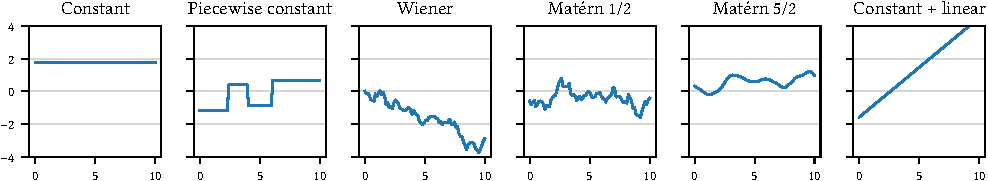
\includegraphics{kks-covariances}
	\caption{Random realizations of a zero-mean Gaussian process with six different covariance functions.}
	\label{kks:fig:covariances}
\end{figure*}

\begin{description}
	\item[Constant] This covariance captures processes that remain constant over time.
	      It is useful in composite covariances to model a constant offset (i.e., a mean score value).

	\item[Piecewise Constant]
	      Given a partition of $\mathbf{R}$ into disjoint intervals, this covariance is constant inside a partition and zero between partitions.
	      It can, for instance, capture discontinuities across seasons in professional sports leagues.

	\item[Wiener] This covariance reflects Brownian motion dynamics (c.f. Section~\ref{kks:sec:relwork}).
	      It is non-stationary: the corresponding process drifts away from $0$ as $t$ grows.

	\item[Matérn] This family of stationary covariance functions can represent smooth and non-smooth variations at various timescales.
	      It is parametrized by a variance, a characteristic timescale and a smoothness parameter $\nu$.
	      When $\nu = 1/2$, it corresponds to a mean-reverting version of Brownian motion.

	\item[Linear] This covariance captures linear dynamics.
\end{description}

% Composite covariance functions.
Finally, note that composite functions can be created by adding or multiplying covariance functions together.
For example, let $k_a$ and $k_b$ be constant and Matérn covariance functions, respectively.
Then, the composite covariance $k(t, t') \doteq k_a(t, t') + k_b(t, t')$ captures dynamics that fluctuate around a (non-zero) mean value.
\citet[Sec. 2.3]{duvenaud2014automatic} provides a good introduction to building expressive covariance functions by composing simple ones.

%! TEX root = ../thesis.tex
\section{Experimental Results}
\label{clm:sec:results}

Starting with no information at all, we arbitrarily set the prior noise $\sigma_n^{2} = 1$ and the prior covariance matrix to a spherical covariance $\vec{\Sigma}_p = \sigma_p^{2} \vec{I}$, with $\sigma_p^{2} = 10$.
Our results are qualitatively robust to a large range of values for $\sigma_p^{2}$.
In order to compare the perceived carbon footprint $\exp \overline{\vec{w}}$ with its true value $\exp \vec{v}$, we set the prior mean to $\vec{\mu} = c \vec{1}$, where $ c = \frac{1}{M}\sum_{i=1}^M v_i$ is the mean of the (log-)true values.
This guarantees that the perceived carbon footprint estimated from the model parameters have the same scale as the true values.

We compile a set $\mathcal{A}$ of $M=18$ individual actions about transportation, food, and household (the full list of actions is provided in Appendix~\ref{clm:app:actions}).
We deploy an online quiz\footnote{Accessible at \url{http://www.climpact.ch}} to collect pairwise comparisons of actions from real users on a university campus.
We collect $N=2183$ triplets from 176 users, mostly students between 16 and 25 years old.
We show in Figure~\ref{clm:fig:perception} the true carbon footprint, together with the global perception of the population, \textit{i.e.}, the values $\exp \overline{w}_i$ for each action $i \in \mathcal{A}$.

\begin{figure}
	\centering
	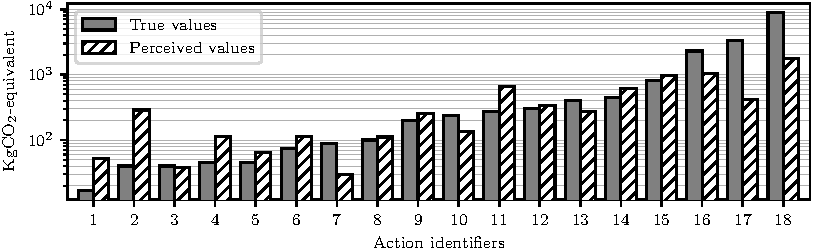
\includegraphics[width=\textwidth]{clm-perception}
	\caption{Global perceived carbon footprint of 18 actions in kg\COtwo-equivalent and their true values (log scale).
		The list of actions is provided in Appendix~\ref{clm:app:actions}.}%
	\label{clm:fig:perception}
\end{figure}

The users in our population have a globally accurate perception.
Among the actions showing the most discrepancy, the carbon footprint of short-haul flights is \textit{overestimated}~(Action 11), whereas the carbon footprint of long-haul flights~(16) is highly \textit{underestimated}~(the scale is logarithmic).
Similarly, the carbon footprint of first-class flights~(18) is also \textit{underestimated}.
The users tend to \textit{overestimate} the carbon footprint of more ecological transports, such as the train, the bus, and car-sharing~(1, 4, and 6).
The users have an accurate perception of actions related to diet~(8, 14, and 15) and of actions related to domestic lighting~(3 and 10).
They \textit{overestimate}, however, the carbon footprint of a dryer~(2).
Finally, they highly \textit{underestimate} the carbon footprint of oil heating~(17).
Switzerland, where the users live, is one of the European countries whose consumption of oil for heating houses is the highest.
There is, therefore, a high potential for raising awareness around this issue.

\input{4-conclusion}

\newpage
\bibliographystyle{abbrvnat}
\bibliography{climpact}

\appendix
%! TEX root = ../thesis.tex
\section{Appendix}

% \subsection{Scaling the Parameters}
% \label{app:scaling}

% The perceived carbon footprints $\exp \overline{\vec{w}}$ have no unit.
% We scale them in order to compare with the true values.
% Let $\vec{v} \in \mathbf{R}^M$ be the true values of the carbon footprint of actions, and $\widetilde{\vec{v}} = \log{\vec{v}}$.
% We want to find the scaling constant $c \in \mathbf{R}$ that minimizes
% \begin{equation*}
%   l(c) = \sum_{i=1}^{M}(\widetilde{v}_i-\overline{w}_i - c)^2.
% \end{equation*}
% We take the derivative of $l(c)$ with respect to $c$ and set it to zero, to obtain
% \begin{equation*}
%   c = \frac{1}{M}\sum_{i=1}^{M} (\widetilde{v}_i - \overline{w}_i).
% \end{equation*}
% Hence, we obtain the scaled perceived carbon footprint of actions $\exp{(\overline{\vec{w}})}\exp{(c)}$.

\subsection{Total Information Gain for Multivariate Gaussian Distributions}
\label{app:active_learning}

Recall that the entropy of a multivariate Gaussian distribution $ \mathcal{N}(\vec{\mu}, \vec{\Sigma}) $, $\vec{\mu} \in \mathbf{R}^M$, $\vec{\Sigma} \in \mathbf{R}^{M \times M}$, is given by
\begin{equation}
	S = \frac{M}{2}(1 + \log 2 \pi) + \frac{1}{2} \log \det \vec{\Sigma}.
\end{equation}
Let $\vec{\Sigma}_N$ and  $\vec{\Sigma}_{N+1}$ be the covariance matrices of the posterior distribution in Equation~\eqref{eq:posterior} when $N$ and $N+1$ data points have been collected, respectively.
Let $\vec{x}$ be the new $(N+1)$-th data point.
The total information gain is
\begin{eqnarray}
	\Delta S &=& S_N - S_{N+1}  \nonumber \\
	&=& \frac{1}{2} \log \frac{\det \vec{\Sigma}_{N+1}^{-1}}{\det \vec{\Sigma}_N^{-1}} \nonumber \\
	&=& \frac{1}{2} \log \frac{\det [\vec{\Sigma}_N^{-1} + \sigma_n^{-2}\vec{x}\vec{x}\tr] }{\det \vec{\Sigma}_N^{-1}} \label{eq:covariance} \\
	&=& \frac{1}{2} \log \frac{(\det \vec{\Sigma}_N^{-1})(1 + \sigma_n^{-2} \vec{x}\tr \vec{\Sigma}_N \vec{x} ) }{ \det \vec{\Sigma}_N^{-1} } \label{eq:determinant} \\
	&=& \frac{1}{2} \log (1 + \sigma_n^{-2} \vec{x}\tr \vec{\Sigma}_N \vec{x}). \nonumber
\end{eqnarray}
We obtain Equation~\eqref{eq:covariance} by observing that $ \vec{\Sigma}_N^{-1} + \sigma_n^{-2} \vec{x} \vec{x}\tr = \sigma_n^{-2} \vec{X}\tr \vec{X} + \vec{\Sigma}_p^{-1} + \sigma_n^{-2} \vec{x} \vec{x}\tr = \vec{\Sigma}_{N+1}^{-1}$.
We obtain Equation~\eqref{eq:determinant} by the matrix determinant lemma.

\subsection{List of Actions}
\label{app:actions}

We provide here the full list of actions, together with the true carbon footprint associated with each of them.
Because different countries use different sources of energy, we calculate the carbon footprint \textit{relative} to the country where our university is located.
The actions are ordered according to their true carbon footprint.
\begin{enumerateb}
	\item \actiontitle{Take the train in economy class on a 1000-km round-trip.} \\
	The train is a high-speed train with 360 seats.
	The seat-occupancy rate is 55\% (average rate for these types of trains).
	We count the \COtwo\ emissions per passenger. \\
	\actionvalue{17} % \cite{sncf2019calcul}
	\item \actiontitle{Dry your clothes with a dryer for one year.} \\
	A dryer emits \COtwo\ because it consumes electricity.
	We consider a dryer of average quality.
	The electricity is consumed from a grid with average \COtwo\ rate. \\
	\actionvalue{40} % \cite{wynes2017climate}
	\item \actiontitle{Light your house with LED bulbs.} \\
	LED bulbs emit CO2 because they consume electricity to generate light.
	The electricity is consumed from a grid with average \COtwo\ rate. \\
	\actionvalue{40} % [Appendix \ref{app:bulbs}]
	\item \actiontitle{Take the bus on a 1000-km round-trip.} \\
	The bus is a standard-size bus with 60 seats.
	The seat-occupancy rate is 50\% (average rate for buses).
	We count the \COtwo\ emissions per passenger. \\
	\actionvalue{45} % \cite{mobitool,myclimate}
	\item \actiontitle{Drive an electric car alone on a 1000-km round-trip.} \\
	The car is a compact electric car that consumes 15 kWh/100km.
	The electricity is consumed from a grid with average \COtwo\ rate.
	There are no other passengers in the car.
	We count the \COtwo\ emissions per passenger. \\
	\actionvalue{45} % \cite{ofdl,myclimate,swissc02}
	\item \actiontitle{Car-share with three other persons on a 1000-km round-trip.} \\
	The car is a mid-sized gasoline car that consumes 7 l/100km.
	There are four persons in the car.
	We count the \COtwo\ emissions per passenger. \\
	\actionvalue{75} % \cite{ofdl,myclimate}
	\item \actiontitle{Eat local and seasonal fruits and vegetables for one year.} \\
	Growing food emits \COtwo\ because it requires fertilizing and driving agricultural machines.
	The goods are then transported to grocery shops and to your home. \\
	\actionvalue{89} % \cite{swissveg,foodmile}
	\item \actiontitle{Eat eggs and dairy products for one year.} \\
	The production of eggs and dairy products (milk, cheese, etc.) emits \COtwo\ because of water and land consumption, animal methane, and fossil fuel consumption for transportation and heating.
	We consider an average citizen consuming 50 kg of eggs and dairy products per year. \\
	\actionvalue{100} % \cite{wynes2017climate,viandesuisse}
	\item \actiontitle{Throw all waste in the same trash for one year.} \\
	Throwing all waste (PET, glass, cardboard, etc.) in the same trash, i.e., without recycling, emits \COtwo\ because more energy is needed to extract, transport, and process raw materials.
	Incinerators also burn more waste, and organic waste decomposition generates methane. \\
	\actionvalue{200} % \cite{wynes2017climate}
	\item \actiontitle{Light your house with incandescent bulbs.} \\
	Incandescent bulbs emit \COtwo\ because they consume electricity to generate light.
	The electricity is consumed from a grid with average \COtwo\ rate. \\
	\actionvalue{239} % [Appendix \ref{app:bulbs}]
	\item \actiontitle{Fly in economy class for a 800-km round-trip.} \\
	The plane is a standard aircraft for short-distance flights with 180 seats.
	The seat-occupancy rate is 80\%.
	We count the \COtwo\ emissions per passenger. \\
	\actionvalue{270} % \cite{bofinger2013calculating,myclimate}
	\item \actiontitle{Drive alone for a 1000-km round-trip.} \\
	The car is a mid-sized gasoline car that consumes 7 l/100km.
	There are no other passengers in the car.
	We count the \COtwo\ emissions per passenger. \\
	\actionvalue{300} % \cite{mobitool,myclimate}
	\item \actiontitle{Heat your house with a heat pump for one year.} \\
	A heat pump emits \COtwo\ because it consumes electricity to generate heat.
	The house is of average size.
	The electricity is consumed from a grid with average \COtwo\ rate. \\
	\actionvalue{400} % \cite{energyenvironnement,swissenergyscope,swissc02}
	\item \actiontitle{Eat imported and out-of-season fruits and vegetables for one year.} \\
	Growing food emits \COtwo\  because it requires fertilizing and driving agricultural machines.
	Importing food emits \COtwo\ because of fossil fuel consumption for transportation.
	Out-of-season food emits \COtwo\ because it grows in greenhouse that needs to be heated.
	The goods are then transported to grocery shops and to your home. \\
	\actionvalue{449} % \cite{foodmile,swissveg}
	\item \actiontitle{Eat meat for one year.} \\
	Meat production emits \COtwo\ because of water and land consumption, animal methane, and fossil fuel consumption for transportation and heating.
	We consider an average citizen consuming 50 kg of meat per year. \\
	\actionvalue{800} % \cite{wynes2017climate,viandesuisse}
	\item \actiontitle{Fly in economy class for a 12000-km round-trip.} \\
	The plane is a standard aircraft for long-distance flights with 390 seats.
	The seat-occupancy rate is close to 100\%.
	We count the \COtwo\ emissions per passenger. \\
	\actionvalue{2300} % \cite{bofinger2013calculating,myclimate}
	\item \actiontitle{Heat your house with an oil furnace for one year.} \\
	An oil furnace emits \COtwo\ because it burns fuel to generate heat.
	The house is of average size. \\
	\actionvalue{3300} % \cite{energyenvironnement,swissenergyscope}
	\item \actiontitle{Fly in first class for a 12000-km round-trip.} \\
	The plane is a standard aircraft for long-distance flights with 390 seats.
	The seat-occupancy rate is close to 100\%.
	We count the \COtwo\ emissions per passenger.
	Passengers flying in first class use more space than passengers in economy. \\
	\actionvalue{9000} % \cite{bofinger2013calculating,myclimate}
\end{enumerateb}


\end{document}
